\chapter{Design and implementation}\label{chap:design}

	For implementation, we use two programming languages - Java and Python. The application is a console one, running firstly on Linux (see Chapter \ref{chap:requirements}, Section \ref{sec:server_param}), even though due to the languages chosen it runs on MS Windows without problems as well.
	
	We use several Java libraries and Python modules which allow for quicker and more efficient execution of many needed tasks.
	
	Java libraries:	
\begin{itemize}
	\item Commons Math: The Apache Commons Mathematics Library - used for all calculations related to SLR and other mathematical requirements,
	\item eap.fits - a NASA Java interface to FITS files, allowing for opening, reading and manipulating FITS files.
\end{itemize}		

	And Python modules:
\begin{itemize}
	\item Astropy - a module for performing astronomy and astrophysics related tasks in Python,
	\item tflearn - a deep learning higher-level library.
\end{itemize}

	Throughout the document, you can see many classes having the prefix \emph{SDT} - it stands for \emph{space debris tracklet} and besides marking the classes as our own and distinguishing them from the rest means nothing.

\section{Classes}\label{sec:classes}

	There more than 10 Java classes (along with the Main class) in our implementation.
	
	Classes which are not covered in detail in this document are:
	
\begin{itemize}
	\item Rectascension - class responsible for holding information about RA of an object and converting it to degrees
	\item Declination - class responsible for holding information about Dec of an object and converting it to degrees
	\item Type - enumeration of all possible types of an object
	\item Arguments - class for matching arguments in command line/terminal
	\item Combinations - class responsible for calculating all possible combinations of three objects out of \emph{n} objects
\end{itemize}

	All the other classes - their member variables and methods - are described in the next subsections.
	
\subsection{algorithms.SDTLinearRegression}\label{subsec:slr}

	A class responsible for handling SLR. It contains all user-set values denoting thresholds needed for fine-tuning accuracy of the SLR described in Chapter \ref{chap:proposed_solutions}, Section \ref{sec:linear_regression}.
	
\begin{table}[H]
\centering
\setlength{\extrarowheight}{2pt}
\begin{tabularx}{\textwidth}{|X|X|}
\hline
\textbf{Class variable} & \textbf{Description} \\ \hline
private static final double \mbox{distanceThreshold} & a double representing distance threshold \\ \hline
private static final double \mbox{angleThreshold} & a double representing angle threshold    \\ \hline
private static final double \mbox{speedThreshold} & a double representing speed threshold    \\ \hline
\end{tabularx}
\caption{SDTLinearRegression class variables table}
\label{tab:class_variables_LR}
\end{table}

\begin{table}[H]
\centering
\setlength{\extrarowheight}{2pt}
\begin{tabularx}{\textwidth}{|X|X|}
\hline
\textbf{Method} & \textbf{Description} \\ \hline
public static void \mbox{perform} & a method responsible for performing all necessary actions, called from outside of the class \\ \hline
private static void \mbox{findInitialRegressions} & a method responsible for constructing initial regressions from starting points\\ \hline
private static void \mbox{fitPointsToRegressions} & a method responsible for handling all existing SLRs - modifying them, correcting them, etc.\\ \hline
\end{tabularx}
\caption{SDTLinearRegression methods table}
\label{tab:class_methods_LR}
\end{table}

\subsection{algorithms.SDTOrbitDetermination}

	A class wrapping already existing implementation of IOD. It handles translating information from previous steps and passing them to the IOD algorithms described in .
	
\begin{table}[H]
\centering
\setlength{\extrarowheight}{2pt}
\begin{tabularx}{\textwidth}{|X|X|}
\hline
\textbf{Class variable} & \textbf{Description} \\ \hline
private static final double \mbox{AGOLON} & a constant describing longitude of AGO \\ \hline
private static final double \mbox{AGOLAT} & a constant describing latitude of AGO\\ \hline
private static final double \mbox{AGOALT} & a constant describing altitude of AGO\\ \hline
\end{tabularx}
\caption{SDTOrbitDetermination class variables table}
\label{tab:class_variables_OD}
\end{table}

\begin{table}[H]
\centering
\setlength{\extrarowheight}{2pt}
\begin{tabularx}{\textwidth}{|X|X|}
\hline
\textbf{Method} & \textbf{Description} \\ \hline
public static void \mbox{perform} & a method responsible for performing all necessary actions, called from outside of the class \\ \hline
private static void \mbox{transformObjectsIntoObservations} & a method responsible for translating inner objects into Observations (class in the existing implementation of IOD)\\ \hline
\end{tabularx}
\caption{SDTOrbitDetermination methods table}
\label{tab:class_methods_OD}
\end{table}

\subsection{SDTObject}\label{subsec:object}

	The SDTObject class is responsible for representing a single object in our implementation. SDTObjects are created while parsing and reading FITS and .cat files and contain several vitally important variables and methods for saving and calculating mandatory data.
	
\begin{table}[H]
\centering
\setlength{\extrarowheight}{2pt}
\begin{tabularx}{\textwidth}{|X|X|}
\hline
\textbf{Class variable} & \textbf{Description} \\ \hline
private String \mbox{fileName} & a String variable containing the name of the file in which the object resides (same for both FITS and .cat files) \\ \hline
private Type \mbox{type} & enumerator marking type of the object (see\ref{} \\ \hline
private \mbox{Rectascension} \mbox{rectascension} & custom data structure holding information about RA of the object \\ \hline
private \mbox{Declination} \mbox{declination} & custom data structure holding information about Dec of the object \\ \hline
private double \mbox{magnitude} & double representing magnitude of the object \\ \hline
private double \mbox{x} & \emph{x} value of the object on the reference frame \\ \hline
private double \mbox{y} & \emph{y} value of the object on the reference frame \\ \hline
private double \mbox{mjd} & double containing date in the Modified Julian Date \\ \hline
private double \mbox{xComponent} & the unified variable containing either RA value or \emph{x} value \\ \hline
private double \mbox{yComponent} & the unified variable containing either Dec value or \emph{y} value \\ \hline
\end{tabularx}
\caption{SDTObject class variables}
\label{tab:class_variables_O}
\end{table}

\begin{table}[H]
\centering
\setlength{\extrarowheight}{2pt}
\begin{tabularx}{\textwidth}{|X|X|}
\hline
\textbf{Method} & \textbf{Description} \\ \hline
public \mbox{SDTObject} & constructor for the SDTObject class \\ \hline
public double \mbox{calculateDistanceToLine} & method which takes a regression as a parameter and calculates distance of the object to the trend line \\ \hline
public boolean \mbox{isWithinLineThreshold} & method returning whether the object is in the pre-determined \emph{distanceThreshold} \\ \hline
public double \mbox{calculateDeltaTime} & method subtracting time of an another object and returning delta time \\ \hline
public double \mbox{calculateSpeed} & method calculating speed \\ \hline
public boolean \mbox{isWithinSpeedThreshold} & method returning boolean value representing whether the object is in the \emph{speedThreshold} variable \\ \hline
public double \mbox{calculateHeading} & method calculating heading \\ \hline
public boolean \mbox{isWithinAngleThreshold} & method deciding whether the object is in the \emph{angleThreshold} \\ \hline
public int \mbox{compareTo} & overridden method from the Comparable<SDTObject> interface implemented by the class \\ \hline
public String \mbox{shortString} & convenience method constructing a short String containing only few information about the object \\ \hline
public String \mbox{verboseString} & convenience method constructing a long String containing significant number of information about the object \\ \hline
public String \mbox{toString} & convenience method returning either short or verbose String, depending on the internal switch \\ \hline
public boolean \mbox{isUnidentified} & method which determines whether an object is unknown or not (Types \emph{H}, \emph{S} and \emph{U} \\ \hline
private double \mbox{produceMjd} & method converting the time read from a FITS file header into MJD \\ \hline
public void \mbox{setTime} & method setting the MJD time gotten from the \emph{produceMJD} method \\ \hline
\end{tabularx}
\caption{SDTObject methods table}
\label{tab:class_methods_O}
\end{table}

	Besides all the methods mentioned in the Table \ref{tab:class_methods_O}, the class also contains setter and getter for every private variable mentioned in the Table \ref{tab:class_variables_O}.

\subsection{SDTBatch}\label{subsec:batch}

	A class used to hold and keep general information and data in the application, such as all existing SLRs, objects and tracklets and containing getters and setters for the mentioned data structures. Few convenience methods for better human readability are present as well.
	
\begin{table}[H]
\centering
\setlength{\extrarowheight}{2pt}
\begin{tabularx}{\textwidth}{|X|X|}
\hline
\textbf{Class variable} & \textbf{Description} \\ \hline
private \mbox{Set<SDTObject> fSet} & the first set of objects (from the first FITS file and the first .cat file) \\ \hline
private \mbox{Set<SDTObject> sSet} & the second set of objects \\ \hline
private \mbox{List<SDTObject> data} & a list containing the rest of the objects from the rest of the files \\ \hline
private \mbox{Map<ArrayList<SDTObject>,} \mbox{SimpleRegression> regressions} & the Commons Math library's implementation of SLR does not allow for retrieving input data so we implement this map to keep track of them \\ \hline
private \mbox{List<SDTObject> regressionResults} & a list containing final tracklet \\ \hline
public static \mbox{Map<String, Integer> objectsCount} & a helper map for keeping track of number of objects in each file \\ \hline
public static \mbox{HashSet<SDTTracklet> tracklets} & a set containing all tracklets \\ \hline
public static final boolean \mbox{DEBUG} & a switch to mark whether application should run in debug mode \\ \hline
public static final boolean \mbox{RADEC} & a switch to resolve if we wish the application to use RA/Dec \\ \hline
\end{tabularx}
\caption{SDTBatch class variables table}
\label{tab:class_variables_B}
\end{table}

\begin{table}[H]
\centering
\setlength{\extrarowheight}{2pt}
\begin{tabularx}{\textwidth}{|X|X|}
\hline
\textbf{Method} & \textbf{Description} \\ \hline
public \mbox{SDTBatch} & constructor initializing empty \emph{regressions}, \emph{data}, \emph{fSet} and \emph{sSet} \\ \hline
public void \mbox{mainDataInsert} & a method for inserting \mbox{SDTObjects} into \emph{data} \\ \hline
public void \mbox{firstSetInsert} & a method for inserting \mbox{SDTObjects} into \emph{fSet} \\ \hline
public void \mbox{secondSetInsert} & a method for inserting \mbox{SDTObjects} into \emph{sSet} \\ \hline
public \mbox{Set<SDTObject> getFirstSet} & getter for the set containing first objects \\ \hline
public \mbox{Set<SDTObject> getSecondSet} & getter for the second set \\ \hline
public \mbox{List<SDTObject> getMainData} & getter for the \emph{data} list \\ \hline
public \mbox{Map<ArrayList<SDTObject,} \mbox{SimpleRegression getRegressions} & getter for the \emph{regressions} map \\ \hline
public void \mbox{setRegressionResults} & setter for inserting the final tracket \\ \hline
public \mbox{List<SDTObject>} \mbox{getRegressionResults} & getter returning the final tracklet \\ \hline
public void \mbox{filterOutEmptyTracklets} & a method which removes tracklets which contain less than three objects and therefore does not conform to the general definition of tracklets \\ \hline
public String \mbox{toString} & a convenience method returning \emph{data} list in String format \\ \hline
\end{tabularx}
\caption{SDTBatch methods table}
\label{tab:class_methods_B}
\end{table}

\subsection{SDTTracklet}\label{subsec:tracklet}

	SDTTracklet is a class which holds objects in a complex structure designed specifically to allow for convenience and performance while handling said objects and accommodates for the SLR algorithm performed in the class \emph{SDTLinearRegression} described in Subsection \ref{subsec:slr}.
	
	The class contains two member variables, specifically \newline \mbox{public ArrayList<ArrayList<Map<SDTObject, Double>{}>{}> objects} \newline and \mbox{public double valueToCompareWith}.
	
	\emph{objects} is a two-dimensional list. The first dimension's length corresponds to the number of all images in the currently processed batch and therefore all possible number of objects a tracklet can contain. The second dimension can be imagined as \emph{bins} which contain every possible object which passes through the filters. The objects in bins are represented as a map with \emph{SDTObject} as the key and Double as the explicit value assigned while calculating a SLR. For more information on this process concerning the filters and the explicit value, see Chapter \ref{chap:proposed_solutions}, Section \ref{sec:linear_regression}. Figure \ref{fig:2dbins} illustrates the \emph{objects} list.
	
	\begin{figure}[H]
	\centering
	  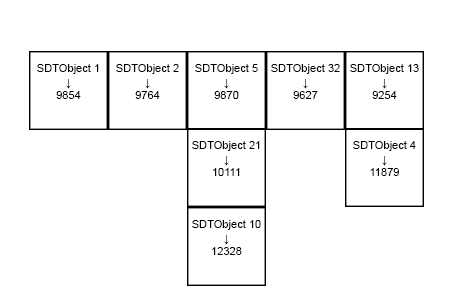
\includegraphics[width=10cm]{images/2dbins}
		  \caption{two-dimensional \emph{objects} list.}
	  \label{fig:2dbins}
	\end{figure}

\begin{table}[H]
\centering
\setlength{\extrarowheight}{2pt}
\begin{tabularx}{\textwidth}{|X|X|}
\hline
\textbf{Method} & \textbf{Description} \\ \hline
pubic \mbox{SDTTracklet} & constructor initialising \emph{objects} list \\ \hline
public SDTObject \mbox{getLastPoint} & method returning the last valid most probable point to insert to the SLR \\ \hline
public void \mbox{sortLast} & method sorting the last non-empty bin according to the Double value in \emph{objects} list \\ \hline
private \mbox{ArrayList<Map<SDTObject,} \mbox{Double>{}> sort} & private method for sorting used by \emph{sortLast} \\ \hline
\end{tabularx}
\caption{SDTTracklet methods table}
\label{tab:class_methods_T}
\end{table}

\subsection{SDTFileHandler}\label{sec:file_handler}

	As the name indicates, this class is responsible for handling files, both FITS and .cat (see Chapter \ref{chap:requirements}, Section \ref{sec:input_data}). We use the mentioned library eap.fits for opening FITS files and reading headers.
	
\begin{table}[H]
\centering
\setlength{\extrarowheight}{2pt}
\begin{tabularx}{\textwidth}{|X|X|}
\hline
\textbf{Method} & \textbf{Description} \\ \hline
static void \mbox{readFiles} & a method responsible for performing all necessary actions and using all utility methods in this class, called from outside of the class \\ \hline
private static void \mbox{insertBatch} & method adding objects to the correct data structure (either \emph{fSet}, \emph{sSet}, or \emph{data}) \\ \hline
private static \mbox{Map<File, File> mergeCATWithFITS} & method internally merging corresponding .cat files with FITS files \\ \hline
private static \mbox{List<File> getCatFiles} & method collecting all the .cat files to be merged \\ \hline
private static \mbox{Map<File, File> mergeCATWithFITS} & method internally merging corresponding .cat files with FITS files \\ \hline
private static \mbox{FitsHeader getFitsHeader} & method returning the header of a FITS file \\ \hline
public static void \mbox{processEntry} & the core method responsible for parsing .cat files, reading FITS headers and creating SDTObjects \\ \hline
\end{tabularx}
\caption{SDTFileHandler methods table}
\label{tab:class_methods_FH}
\end{table}

	Public static methods from the class are used as the first step of the application. Data provided in the files on the disk are read and sent to the next steps.
